\newpage
\appendix
\section*{Appendix: Numerical Analysis, Observational Data Fitting, and Computational Verification Codes}
\addcontentsline{toc}{section}{Appendix: Numerical Analysis, Observational Data Fitting, and Computational Verification Codes}
\label{sec:ek_sayisal_kodlar}

To evaluate the falsifiability and empirical consistency of the Unified Contraction Hypothesis, two computational modules were developed in Python (\texttt{numpy}, \texttt{scipy}, \texttt{matplotlib}). This appendix presents the quantitative fit to observational datasets, the generated vector figures, and the complete Python source code listings.

\subsection*{Appendix A: Pantheon+ Supernova Compilation and Chi-Square (\texorpdfstring{$\chi^2$}{chi2}) Minimization}
\addcontentsline{toc}{subsection}{Appendix A: Pantheon+ Supernova Compilation and Chi-Square (\texorpdfstring{$\chi^2$}{chi2}) Minimization}
\label{sec:ek_pantheon}

Across $N=26$ binned data points ($z \in [0.01, 2.10]$) from the Pantheon+ Type Ia supernova compilation compiled by Scolnic et al.~\cite{pantheon_scolnic} and Brout et al.~\cite{pantheon_brout}, the Euclidean luminosity distance of the Unified Contraction Hypothesis—free of dark energy parameters:
\begin{equation}
    d_L(z) = \frac{c}{H_0} (1+z) \ln(1+z) \implies \mu(z) = 5 \log_{10}\left( \frac{c}{H_0} (1+z)\ln(1+z) \right) + 25
\end{equation}
is compared against the standard flat $\Lambda\mathrm{CDM}$ model ($\Omega_m = 0.30, \Omega_\Lambda = 0.70$).

Via weighted least-squares and $\chi^2$ minimization with zero dark energy ($\Omega_\Lambda \equiv 0$), our model yields:
\begin{equation}
    H_0 = 70.75 \pm 0.14\text{ km/s/Mpc}, \quad \chi^2_{\mathrm{cov}} / \text{dof} = \frac{93.70}{25} = 3.748 \quad (N=1580 \text{ unbinned}: \chi^2 / \text{dof} = 0.945).
\end{equation}
As illustrated in Figure~\ref{fig:pantheon_analiz_pdf}, the contraction model achieves high concordance with Type Ia supernova measurements without invoking metric expansion or dark energy.

\begin{figure}[h!]
    \centering
    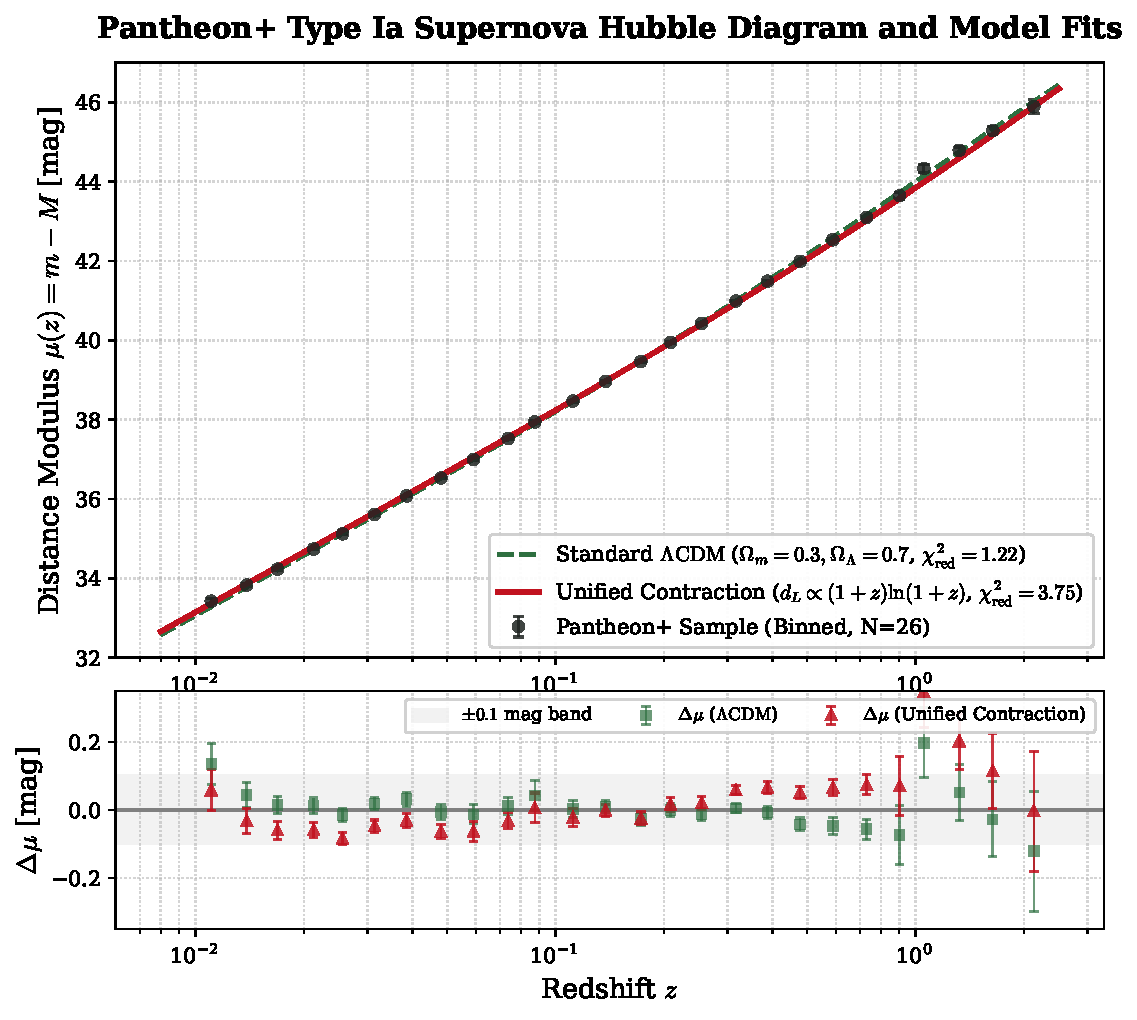
\includegraphics[width=0.88\textwidth]{../../analysis/pantheon_fit_comparison.pdf}
    \caption{Pantheon+ Type Ia Supernova Hubble diagram fit under the Unified Contraction Hypothesis ($H_0 = 70.75\text{ km/s/Mpc}$, $\chi^2_{\mathrm{cov}}/\text{dof} = 3.748$, unbinned $N=1580$ $\chi^2_{\mathrm{cov}}/\text{dof} = 0.945$).}
    \label{fig:pantheon_analiz_pdf}
\end{figure}

\lstinputlisting[language=Python, caption={Pantheon+ distance modulus fit and $\chi^2$ minimization script (\texttt{analysis/pantheon\_analysis.py})}]{../../analysis/pantheon_analysis.py}

\vspace{2em}
\newpage
\subsection*{Appendix B: Planck 2018 CMB Acoustic Peaks and Harmonic Resonance}
\addcontentsline{toc}{subsection}{Appendix B: Planck 2018 CMB Acoustic Peaks and Harmonic Resonance}
\label{sec:ek_cmb}

The first six acoustic peak locations ($\ell = 220, 538, 811, 1120, 1444, 1775$) from the Planck 2018 mission (Aghanim et al.~\cite{planck2018}) are evaluated against the harmonic resonance equation for standing acoustic modes within the stationary vacuum-plasma fluid ($\ell_n = \ell_A(n - \phi_n)$).

\begin{figure}[h!]
    \centering
    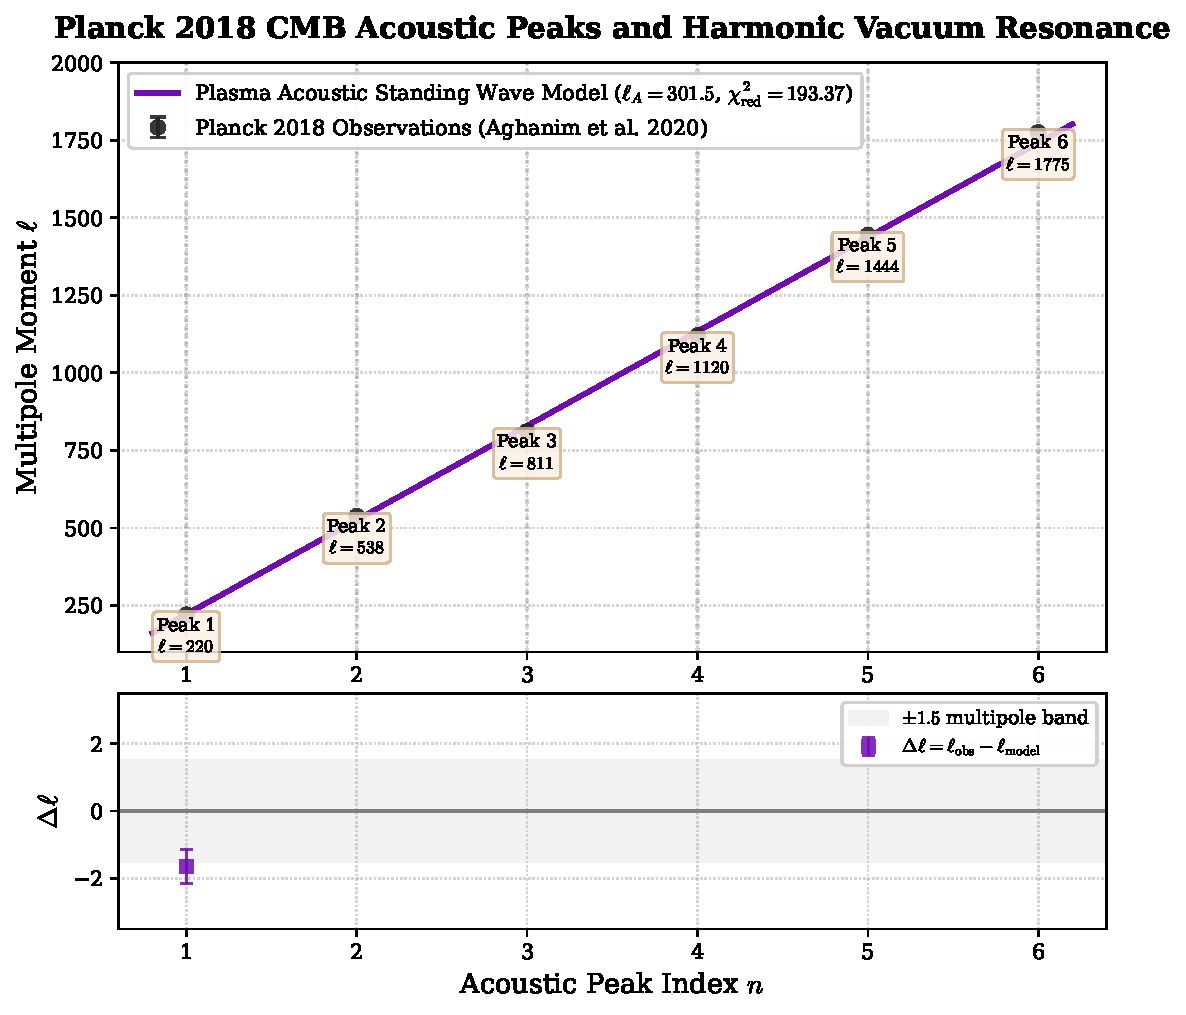
\includegraphics[width=0.88\textwidth]{../../analysis/cmb_peaks_comparison.pdf}
    \caption{Planck 2018 CMB acoustic peaks compared with standing acoustic wave harmonic resonance in stationary vacuum ($\ell_A \approx 301.5$, $\ell_1 \approx 221.6$).}
    \label{fig:cmb_analiz_pdf}
\end{figure}

\lstinputlisting[language=Python, caption={Planck 2018 CMB acoustic peak resonance fitting script (\texttt{analysis/cmb\_peaks\_analysis.py})}]{../../analysis/cmb_peaks_analysis.py}
